\documentclass{article}
\usepackage{colortbl}
\usepackage{fullpage}
\usepackage{times}
\usepackage{booktabs}
\usepackage{bigstrut}
\usepackage{subfig}
\usepackage[table]{xcolor}
\usepackage{graphicx}
\graphicspath{../_fig/}
    \usepackage{picture}
    \newcommand{\quart}[4]{\begin{picture}(100,6)
      {\color{black}\put(#3,3){\circle*{4}}\put(#1,3){\line(1,0){#2}}}\end{picture}}

\begin{document}
\title{Apache}
\date{}
\maketitle 
\begin{table}[h!]
  \centering

{\scriptsize \begin{tabular}{|l@{~~~}|l@{~~~}|r@{~~~}|r@{~~~}|c|}
    \hline
    \textbf{Rank} & \textbf{Treatment} & \textbf{Median} & \textbf{IQR} & \bigstrut\\\hline
    1 & Apache\_25\_w\_iP(75) &    1.0  &  0.03 & \quart{0}{8}{2}{2} \bigstrut\\
    \hline  2 & Apache\_25\_w\_iP(50) &    1.02  &  0.02 & \quart{8}{6}{8}{2} \bigstrut\\
    2 & Apache\_25\_w\_iP(25) &    1.02  &  0.05 & \quart{2}{15}{8}{2} \bigstrut\\
    2 &  Apache\_25\_w &    1.03  &  0.04 & \quart{8}{12}{11}{2} \bigstrut\\
    2 & Apache\_25\_iP(25) &    1.03  &  0.04 & \quart{11}{12}{11}{2} \bigstrut\\
    2 &  Apache\_25\_w &    1.03  &  0.05 & \quart{5}{15}{11}{2} \bigstrut\\
    \hline  3 &  Apache\_25\_w &    1.05  &  0.07 & \quart{11}{21}{17}{2} \bigstrut\\
    3 &    Apache\_25 &    1.06  &  0.03 & \quart{17}{9}{20}{2} \bigstrut\\
    3 & Apache\_25\_iP(75) &    1.07  &  0.06 & \quart{14}{18}{23}{2} \bigstrut\\
    3 & Apache\_25\_iP(50) &    1.07  &  0.03 & \quart{23}{9}{23}{2} \bigstrut\\
    3 &    Apache\_25 &    1.07  &  0.06 & \quart{17}{18}{23}{2} \bigstrut\\
    \hline  4 &  Apache\_50\_w &    1.1  &  0.07 & \quart{23}{21}{32}{2} \bigstrut\\
    4 &    Apache\_25 &    1.1  &  0.02 & \quart{32}{6}{32}{2} \bigstrut\\
    4 & Apache\_50\_w\_iP(75) &    1.1  &  0.04 & \quart{29}{12}{32}{2} \bigstrut\\
    4 &  Apache\_50\_w &    1.1  &  0.09 & \quart{17}{27}{32}{2} \bigstrut\\
    4 &  Apache\_50\_w &    1.12  &  0.03 & \quart{32}{9}{38}{2} \bigstrut\\
    4 & Apache\_50\_w\_iP(25) &    1.13  &  0.07 & \quart{32}{20}{41}{2} \bigstrut\\
    4 & Apache\_50\_w\_iP(50) &    1.14  &  0.07 & \quart{26}{21}{44}{2} \bigstrut\\
    4 &    Apache\_50 &    1.14  &  0.02 & \quart{41}{6}{44}{2} \bigstrut\\
    4 & Apache\_50\_iP(75) &    1.14  &  0.07 & \quart{38}{20}{44}{2} \bigstrut\\
    \hline  5 &    Apache\_50 &    1.15  &  0.1 & \quart{26}{29}{47}{2} \bigstrut\\
    5 & Apache\_50\_iP(50) &    1.17  &  0.06 & \quart{38}{17}{52}{2} \bigstrut\\
    5 & Apache\_50\_iP(25) &    1.17  &  0.06 & \quart{44}{17}{52}{2} \bigstrut\\
    5 &  Apache\_75\_w &    1.18  &  0.07 & \quart{52}{21}{55}{2} \bigstrut\\
    5 & Apache\_75\_w\_iP(75) &    1.19  &  0.05 & \quart{47}{14}{58}{2} \bigstrut\\
    5 &  Apache\_75\_w &    1.19  &  0.11 & \quart{38}{32}{58}{2} \bigstrut\\
    5 &    Apache\_50 &    1.2  &  0.08 & \quart{47}{23}{61}{2} \bigstrut\\
    \hline  6 & Apache\_75\_w\_iP(50) &    1.2  &  0.12 & \quart{47}{35}{61}{2} \bigstrut\\
    6 &  Apache\_75\_w &    1.22  &  0.1 & \quart{52}{30}{67}{2} \bigstrut\\
    6 & Apache\_75\_w\_iP(25) &    1.23  &  0.07 & \quart{67}{21}{70}{2} \bigstrut\\
    \hline  7 &    Apache\_75 &    1.27  &  0.06 & \quart{73}{18}{82}{2} \bigstrut\\
    7 & Apache\_75\_iP(25) &    1.27  &  0.07 & \quart{73}{21}{82}{2} \bigstrut\\
    7 &    Apache\_75 &    1.26  &  0.06 & \quart{79}{18}{79}{2} \bigstrut\\
    7 &    Apache\_75 &    1.29  &  0.08 & \quart{70}{24}{88}{2} \bigstrut\\
    7 & Apache\_75\_iP(50) &    1.29  &  0.05 & \quart{76}{15}{88}{2} \bigstrut\\
    7 & Apache\_75\_iP(75) &    1.31  &  0.06 & \quart{82}{17}{94}{2} \bigstrut\\
    \hline \end{tabular}}
\end{table}
%\begin{figure}
%  \centering
%  
%  \subfloat[][Mutation Probability = 0.25, Feature Weighting, 25\% Information 
%  Pruning Gain($^{Before}/_{
%  After}$)=1.08]{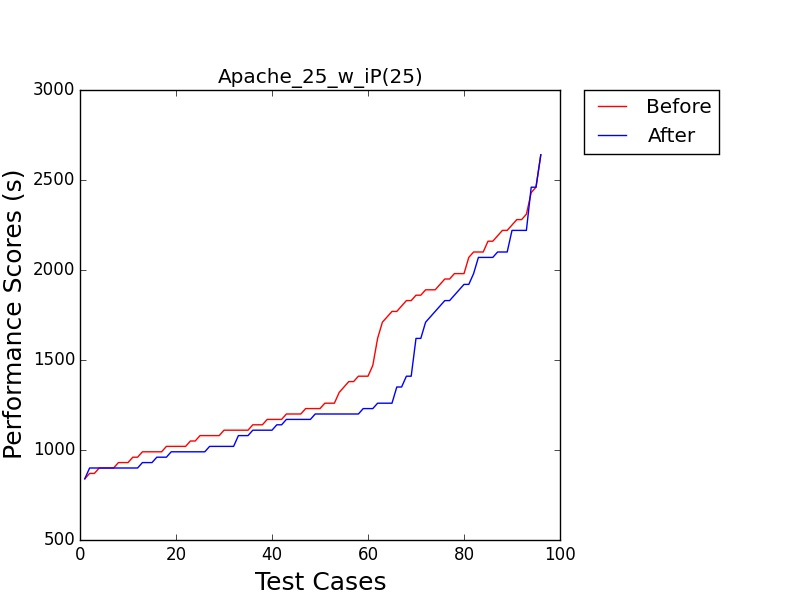
\includegraphics[width=0.8\linewidth]{../_fig/Apache_25_w_iP(25).jpg}\label{}}
%\end{figure} \begin{figure}
%  \centering  
%  \subfloat[][Mutation Probability = 0.25, Feature Weighting, 75\% Information 
%  Pruning Gain($^{Before}/_{
%  After}$)=1.06]{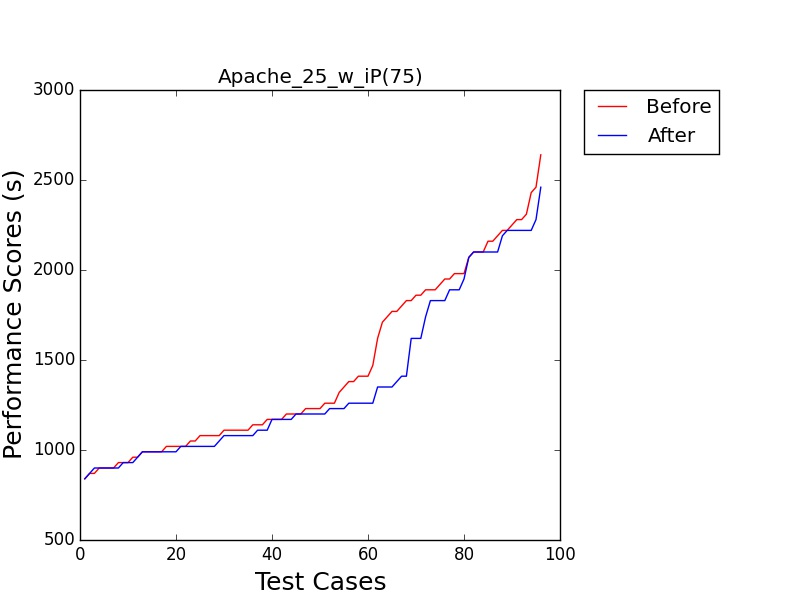
\includegraphics[width=0.8\linewidth]{../_fig/Apache_25_w_iP(75).jpg}\label{}}\\
%  \end{figure} \begin{figure}
%    \centering
%  \subfloat[][Mutation Probability = 0.25, Feature Weighting. Gain($\frac{
%  Before}{
%  After}$)=1.07]{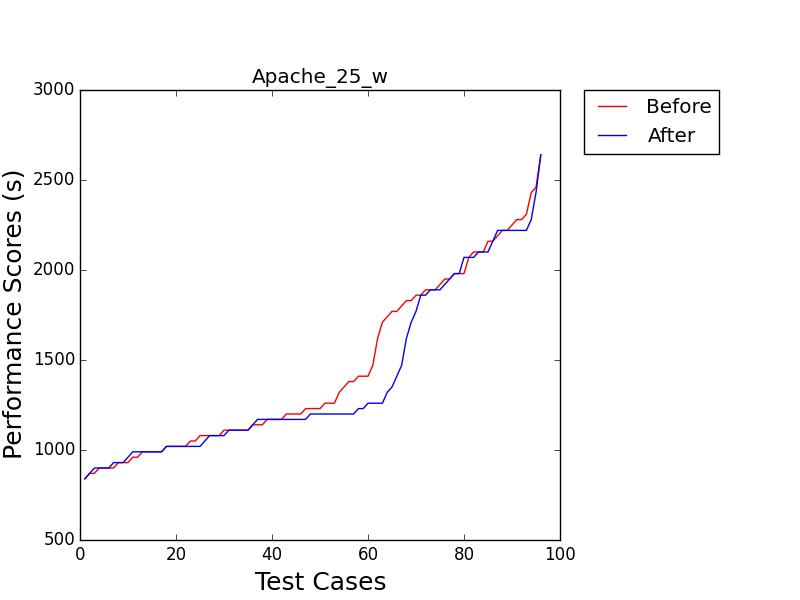
\includegraphics[width=0.8\linewidth]{../_fig/Apache_25_w.jpg}\label{}}
%  \end{figure} \begin{figure}
%    \centering
%  \subfloat[][Mutation Probability = 0.25, Feature Weighting. Gain($\frac{
%  Before}{
%  After}$)=1.04]{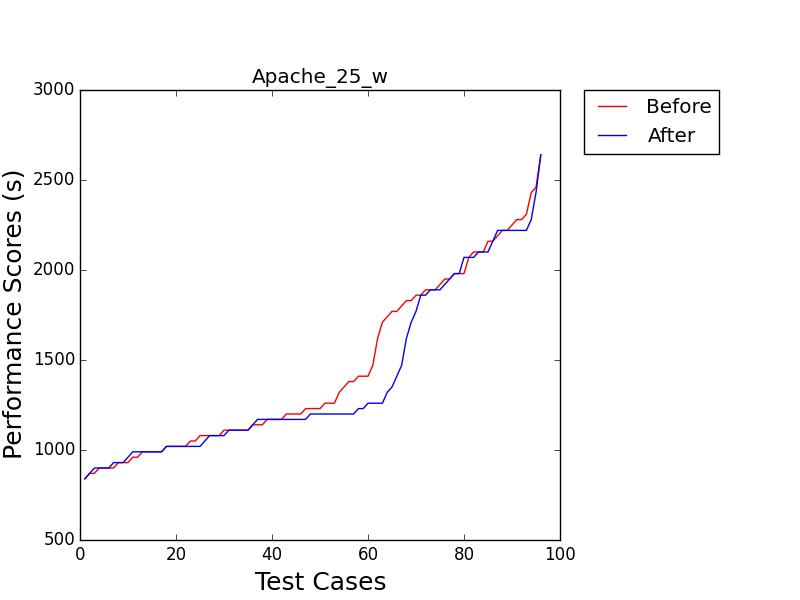
\includegraphics[width=0.8\linewidth]{../_fig/Apache_25_w.jpg}\label{}}\\
%  \end{figure} 
\begin{figure}
    \centering
  \subfloat[][Mutation Probability = 0.75, Feature Weighting, 25\% Information 
  Pruning Gain($^{Before}/_{
  After}$)=1.36]{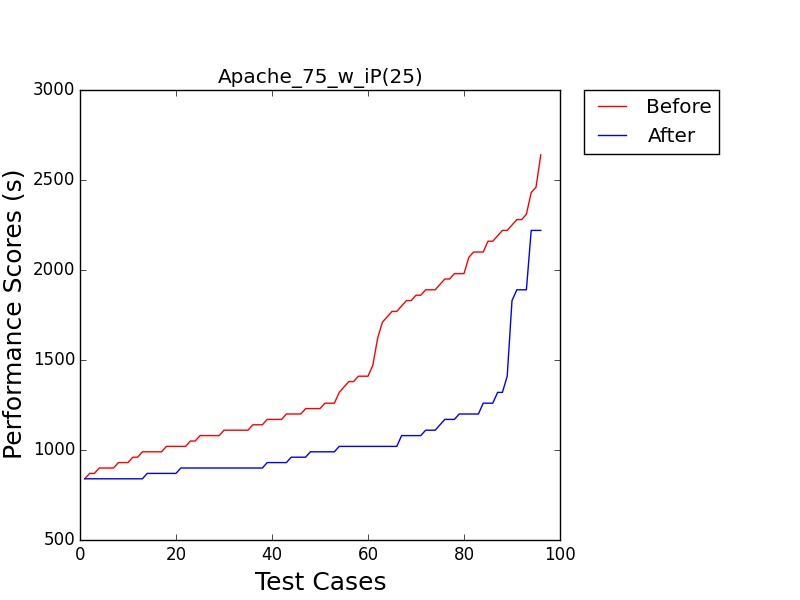
\includegraphics[width=0.8\linewidth]{../_fig/Apache_75_w_iP(25).jpg}\label{}}
 \end{figure} 
%\begin{figure}
%   \centering
% \subfloat[][Mutation Probability = 0.75, Feature Weighting, 75\% Information 
%  Pruning Gain($^{Before}/_{
%  After}$)=1.23]{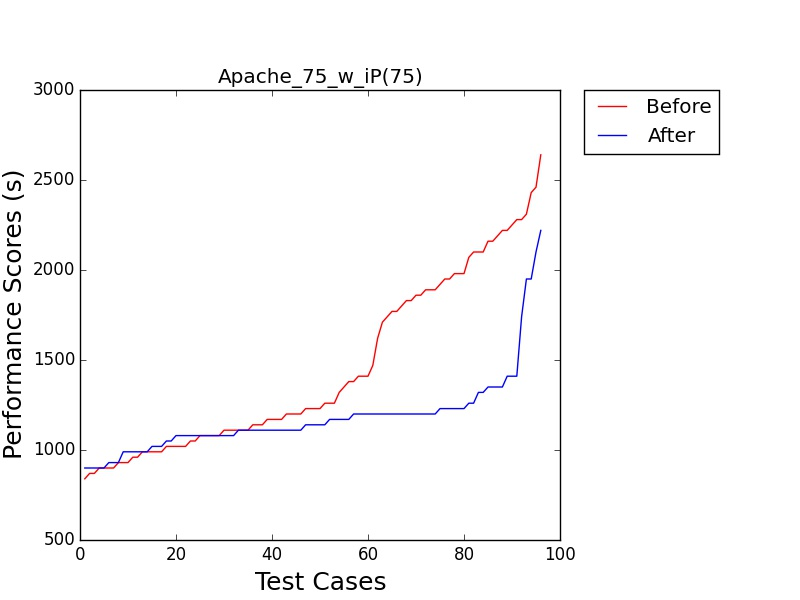
\includegraphics[width=0.8\linewidth]{../_fig/Apache_75_w_iP(75).jpg}\label{}}\\
%  \end{figure} \begin{figure}
%    \centering
%  \subfloat[][Mutation Probability = 0.75, Feature Weighting. Gain($\frac{
%  Before}{
%  After}$)=1.22]{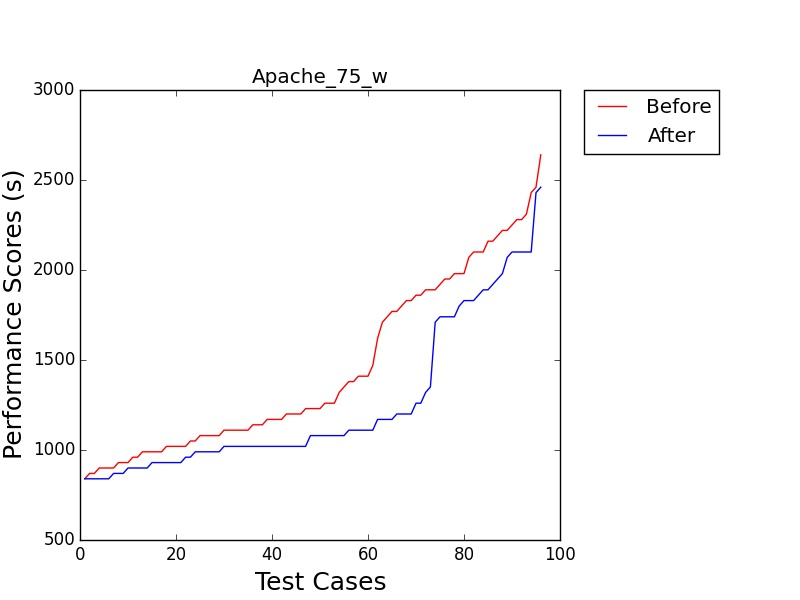
\includegraphics[width=0.8\linewidth]{../_fig/Apache_75_w.jpg}\label{}}
%  \end{figure} \begin{figure}
%    \centering
%  \subfloat[][Mutation Probability = 0.75, Feature Weighting. Gain($\frac{
%  Before}{
%  After}$)=1.16]{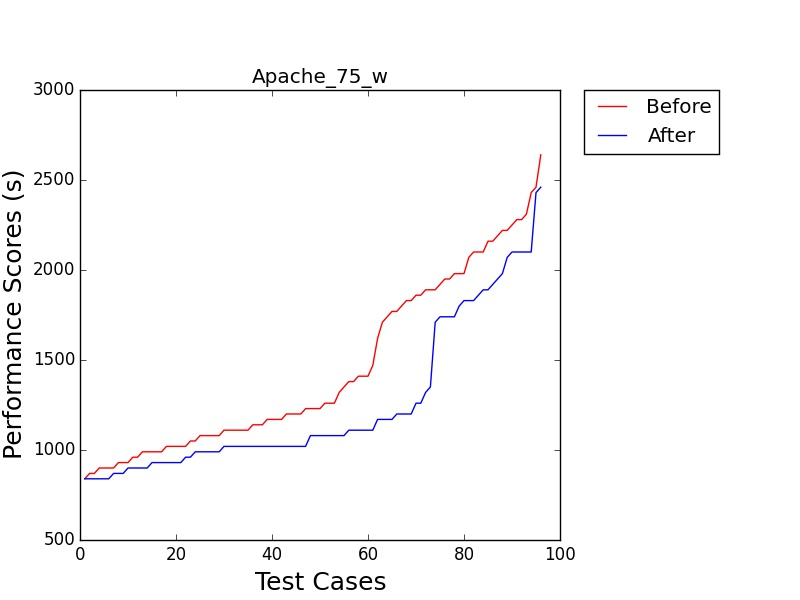
\includegraphics[width=0.8\linewidth]{../_fig/Apache_75_w.jpg}\label{}}\\
%  \end{figure} \begin{figure}
%    \centering
%  \subfloat[][Mutation Probability = 0.25,., 25\% Information Pruning 
%  Gain($^{Before}/_{
%  After}$)=1.07]{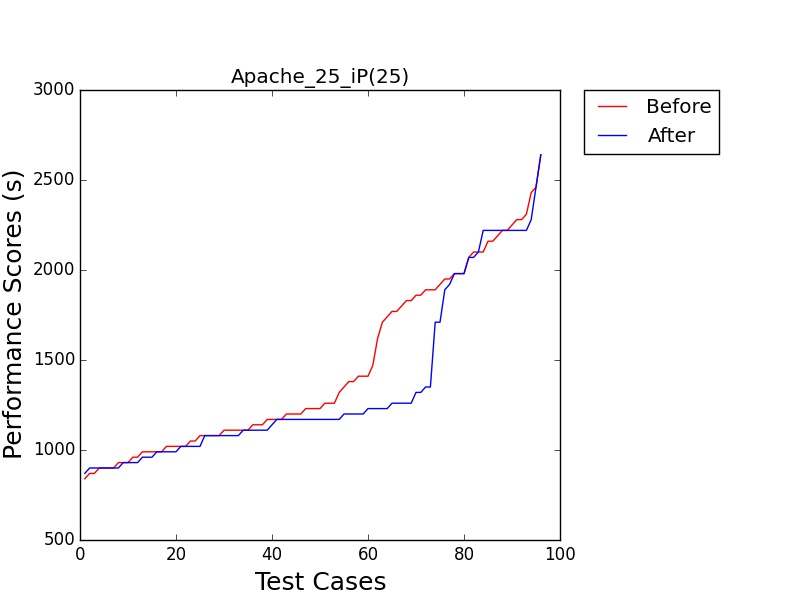
\includegraphics[width=0.8\linewidth]{../_fig/Apache_25_iP(25).jpg}\label{}}
%  \end{figure} \begin{figure}
%    \centering
%  \subfloat[][Mutation Probability = 0.25,., 75\% Information Pruning 
%  Gain($^{Before}/_{
%  After}$)=1.09]{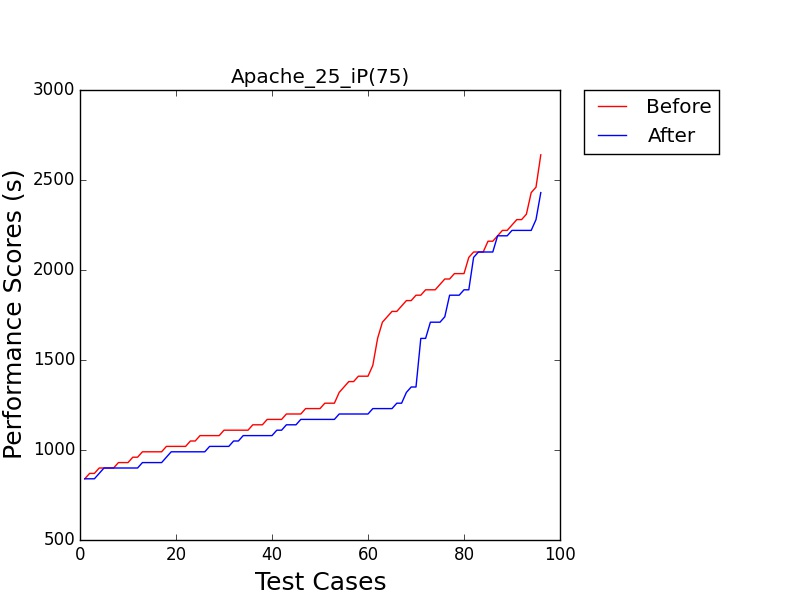
\includegraphics[width=0.8\linewidth]{../_fig/Apache_25_iP(75).jpg}\label{}}\\
%  \end{figure} \begin{figure}
%    \centering
%  \subfloat[][Mutation Probability = 0.25,.. Gain($^{Before}/_{
%  After}$))=1.14]{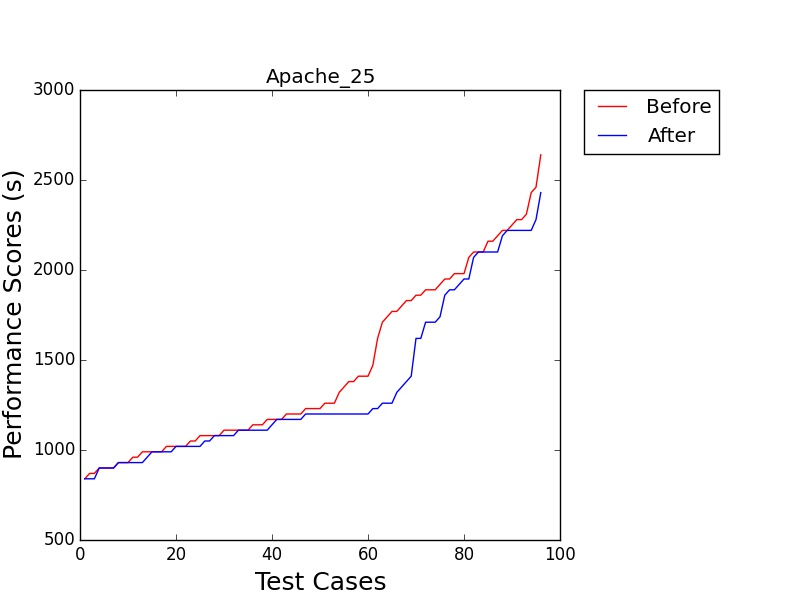
\includegraphics[width=0.8\linewidth]{../_fig/Apache_25.jpg}\label{}}
%  \end{figure} \begin{figure}
%    \centering
%  \subfloat[][Mutation Probability = 0.25,.. Gain($^{Before}/_{
%  After}$)=1.07]{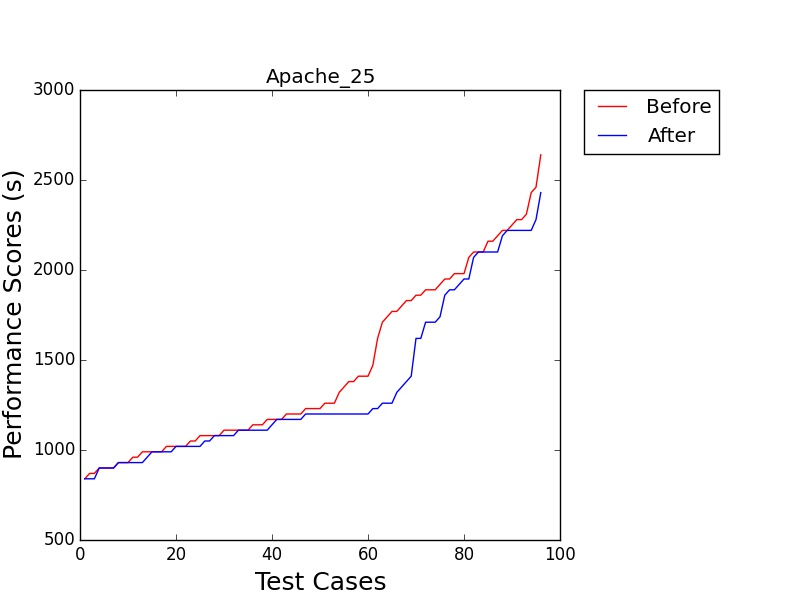
\includegraphics[width=0.8\linewidth]{../_fig/Apache_25.jpg}\label{}}\\
%  \end{figure} 
  \begin{figure}
    \centering
  \subfloat[][Mutation Probability = 0.75, 25\% Information Pruning 
  Gain($^{Before}/_{
  After}$)=1.22]{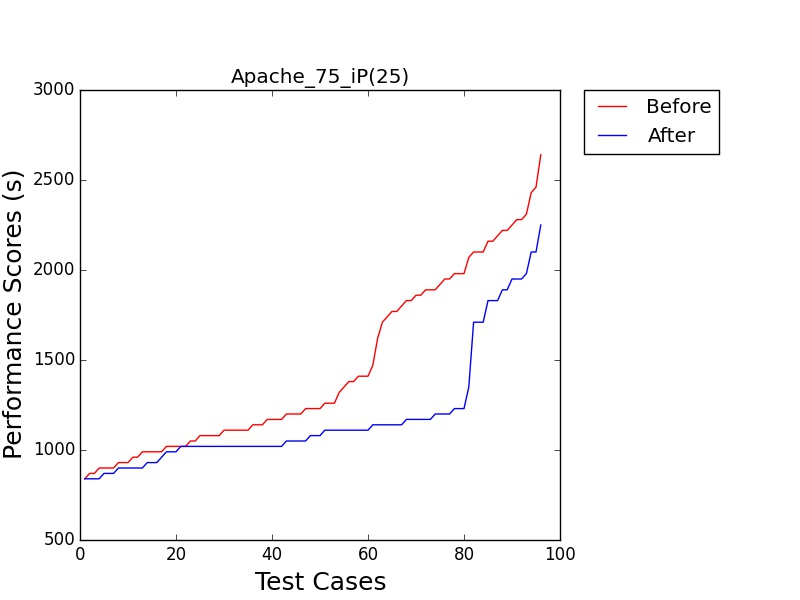
\includegraphics[width=0.8\linewidth]{../_fig/Apache_75_iP(25).jpg}\label{}}
  \end{figure} 
%  \begin{figure}
%    \centering1
%  \subfloat[][Mutation Probability = 0.75,., 75\% Information Pruning 
%  Gain($^{Before}/_{
%  After}$)=1.39]{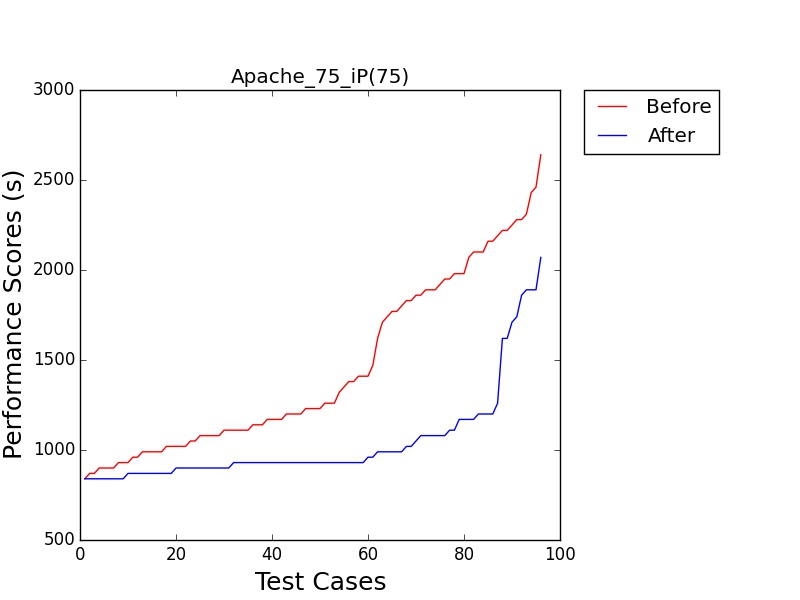
\includegraphics[width=0.8\linewidth]{../_fig/Apache_75_iP(75).jpg}\label{}}\\
%  \end{figure} \begin{figure}
%    \centering
%  \subfloat[][Mutation Probability = 0.75,.. Gain($^{Before}/_{
%  After}$)=1.39]{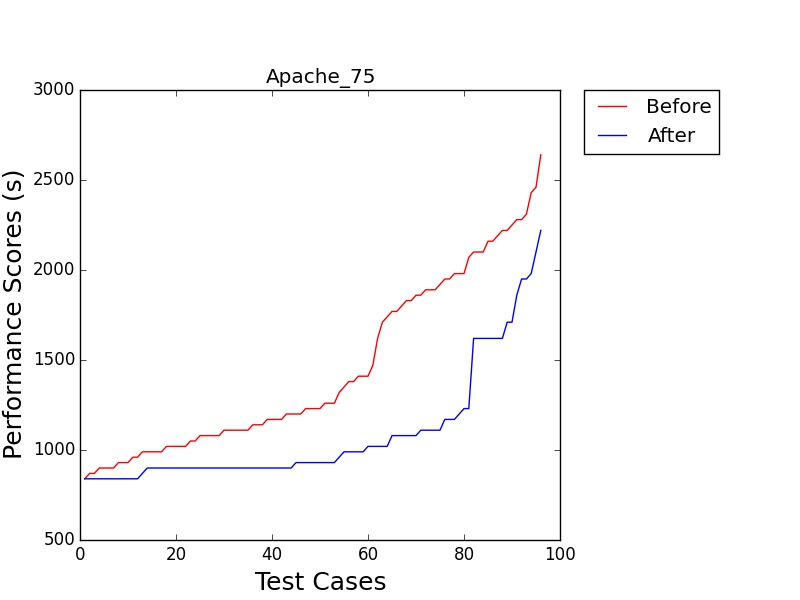
\includegraphics[width=0.8\linewidth]{../_fig/Apache_75.jpg}\label{}}
%  \end{figure} \begin{figure}
%    \centering
%  \subfloat[][Mutation Probability = 0.75,.. Gain($^{Before}/_{
%  After}$)=1.33]{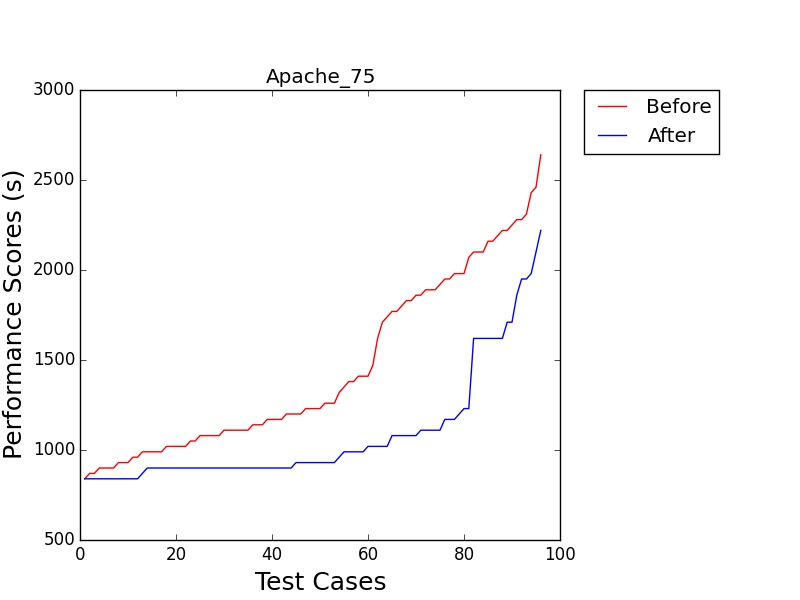
\includegraphics[width=0.8\linewidth]{../_fig/Apache_75.jpg}\label{}}\\
%\end{figure}
\end{document}
